%------- 2.1
\subsection{Conceitos Básicos}
    %--- 2.1.1
    \subsubsection{Definição}
        Conjunto é um agrupamento de elementos, aleatórios ou selecionados criteriosamente por um sistema. Pode ser enumerado ou ter seus critérios descritos em propriedades. \eg
        \[ A = \{ 0,1,2,3,5,8,13 \}; A = \{ x \in \mathbb{U} | \mathcal{P} \} \]
    %--- 2.1.2
    \subsubsection{Tipos}
        \begin{description}
            \item[Conjunto Unitário] é aquele que possui um único elemento. \eg \hfill $ A = \{7\} $
            \item[Conjunto Vazio] é aquele que não possui elemento algum. \eg \hfill $ A = \{  \}; A = \varnothing $
            \item[Conjunto Universo] é aquele que contém todos os elementos utilizados no assunto
tratado
        \end{description}
    %--- 2.1.3
    \subsubsection{Intervalos}
        Definido como uma descrição de conjunto que compreende todos os números em determinado espaço da reta numérica (considerado o conjunto universo), podendo ser abertos ou fechados. \eg
        \[ (a<b) \]
        \[ ]a,b[ = \{ x \in \mathbb{U} | a < x < b \} \]
        \[ [a,b] = \{ x \in \mathbb{U} | a \leq x \leq b \} \]
        
        Intervalos possuem uma representação gráfica na reta numérica. \eg
        \begin{center}
            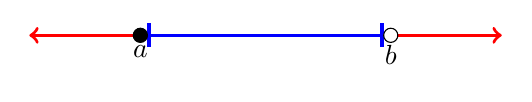
\begin{tikzpicture}
                \draw[red, very thick, <->] (-3,0) -- (3,0);
                \draw[blue, very thick, |-|] (-1.5,0) -- (1.5,0);
                \filldraw[color=black, fill=black] (-1.59,0) circle (0.09) node[below]{$a$};
                \filldraw[color=black, fill=white, thin] (1.59,0) circle (0.09) node[below]{$b$};
            \end{tikzpicture}
            \[ [a,b[ = \{ x \in \mathbb{R} | a \leq x < b \} \]
        \end{center}
    %--- 2.1.4
    \subsubsection{Pares Ordenados}
        Chama-se par ordenado o conjunto de 2 elementos onde sua ordem importa:
        \[ (a,b) = \{ \{ a \}, \{ a, b \} \} \]
        \[ (a,b) = (c,d) \rightarrow a = c \wedge b = d \]
        
        Muito utilizado para a representação de pontos em um plano cartesiano, indicando sua abscissa e sua ordenada, respectivamente:
        \[ P \in \alpha = (x_p, y_p) \]
    %--- 2.1.5
    \subsubsection{Produto Cartesiano}
        Considerando os conjuntos não vazios A e B, o produto cartesiano de A por B é o conjunto cujos elementos são todos os pares ordenados onde o primeiro elemento pertence a A e o segundo a B:
        \[ (A, B \neq \varnothing) \]
        \[ A \times B = \{ (x,y) | x \in A \wedge y \in B \} \]
    %--- 2.1.6
    \subsubsection{Relação Binária}
        A relação binária é um subconjunto criterioso dos elementos de um produto cartesiano definido por uma lei de aplicação:
        \[ R_{A \times B} = \{ (x,y) \in A \times B | \mathcal{P} \} \]
    %--- 2.1.7
    \subsubsection{Domínio}
        Na relação binária de A em B, o domínio é o subconjunto de todos os elementos de A que tenham uma aplicação em B:
        \[ x \in \mathcal{D}(R_{A \times B}) \leftrightarrow \exists y \in B | (x,y) \in R_{A \times B} \]
    %--- 2.1.8
    \subsubsection{Contradomínio}
        Na relação binária de A em B, o contradomínio é simplesmente B, sendo o conjunto de chegada da lei de aplicação:
        \[ \mathcal{CD}(R_{A \times B}) = B \]
    %--- 2.1.9
    \subsubsection{Imagem}
        Na relação binária de A em B, a imagem é o subconjunto do contradomínio formado por todos os elementos que sejam associados ao domínio pela lei de aplicação:
        \[ y \in \mathcal{IM}(R_{A \times B}) \leftrightarrow \exists x \in A | (x,y) \in R_{A \times B} \]
    %--- 2.1.10
    \subsubsection{Relação Inversa}
        Dada a relação binária de A em B, a sua relação inversa é a aplicação de sua lei no produto cartesiano de B por A:
        \[ R^{-1}_{A \times B} = \{ (y,x) \in B \times A | (x,y) \in R_{A \times B} \} \]
%------- 2.2
\subsection{Relações}
    %--- 2.2.1
    \subsubsection{Subconjuntos}
        Um conjunto A é subconjunto de outro conjunto B se todo elemento que pertencente a A também pertence a B:
        \[ A \subset B \leftrightarrow \forall x \in A, B \ni x \]
    %--- 2.2.2
    \subsubsection{Igualdade}
        Dois conjuntos A e B são classificados como iguais quando todo elemento de A pertence a B, e todo elemento de B pertence a A:
        \[ A = B \leftrightarrow (\forall x \in A, B \ni x) \wedge (\forall y \in B, A \ni y) \]
    %--- 2.2.3
    \subsubsection{Reunião}
        Chama-se reunião de A e B o conjunto formado pelos elementos que pertencem a A ou a B:
        \[ A \cup B = \{ x | x \in A \vee x \in B \} \]
    %--- 2.2.4
    \subsubsection{Interseção}
        Chama-se interseção de A e B o conjunto formado pelos elementos que pertencem a A e a B:
        \[ A \cap B = \{ x | x \in A \wedge x \in B \} \]

        Conjuntos que não possuem elementos em comum são chamados conjuntos distintos.
    %--- 2.2.5
    \subsubsection{Diferença}
        Chama-se diferença entre A e B o conjunto formado pelos elementos de A que não pertencem a B:
        \[ A - B = \{ x | x \in A \wedge x \notin B \} \]
    %--- 2.2.6
    \subsubsection{Complementar}
        Considerando um conjunto A e seu subconjunto B, chama-se o complementar de B em relação a A o conjunto dos elementos de A que não pertencem a B:
        \[ (B \subset A) \]
        \[ \mathcal{C}^{B}_{A} = A - B \]
    %--- 2.2.7
    \subsubsection{Propriedades}
        Considerando A, B e C como conjuntos quaisquer:
        \begin{multicols}{3}
            \noindent\[ \varnothing \subset A \]
            \[ A \subset A \]
            \[ A \cup A = A \]
            \[ A \cap A = A \]
            \[ A \cup \varnothing = A \]
            \[ A \cap \varnothing = A \]
            \[ A \cup B = B \cup A \]
            \[ A \cap B = B \cap A \]
            \[ (A \subset B) \wedge (A \supset B) \leftrightarrow A = B \]
            \[ (A \subset B) \wedge (B \subset C) \rightarrow A \subset C \]
            \[ (A \cup B) \cup C = A \cup (B \cup C) \]
            \[ (A \cap B) \cap C = A \cap (B \cap C) \]
        \end{multicols}
        Considerando A e seus subconjuntos B e C:
        \[ (A \supset B,C) \]
        \[ \mathcal{C}^{B}_{A} \cup B = A; \mathcal{C}^{B}_{A} \cap B = \varnothing \]
%------- 2.3
\subsection{Conjuntos Numéricos}
    %--- 2.3.1
    \subsubsection{Naturais}
        O conjunto dos números naturais define-se em:
        \[ \mathbb{N} = \{ 1,2,3,... \} \]
    %--- 2.3.2
    \subsubsection{Inteiros}
        O conjunto dos números inteiros estende o conjunto dos naturais com números negativos:
        \[ \mathbb{Z} = \{ ...,-1,0,1,2,... \} \]
    %--- 2.3.3
    \subsubsection{Racionais}
        O conjunto dos números racionais estende o conjunto dos inteiros com a representação de componentes fracionários:
        \[ \mathbb{Q} = \left\{\frac{a}{b} | a \in \mathbb{Z} \wedge b \in \mathbb{Z}^* \right\} \]
    %--- 2.3.4
    \subsubsection{Irracionais}
        O conjunto dos números irracionais compreende os números da reta numérica que não podem ser representados por frações, sendo dízimas não periódicas sem uma razão numérica:
        \[ \mathbb{I} = \left\{ x | \frac{p}{q} \neq x \ \forall p,q \in \mathbb{Z} \right\} \]
    %--- 2.3.5
    \subsubsection{Reais}
        O conjunto dos números reais engloba todos os números existentes na reta numérica, sendo a união do conjunto dos racionais com o conjunto dos irracionais:
        \[ \mathbb{R} = \mathbb{Q} \cup \mathbb{I} \]
    %--- 2.3.6
    \subsubsection{Imaginários}
        O conjunto dos números imaginários traz o conceito de perpendicularidade para a reta numérica:
        \[ \mathfrak{I} = \left\{ \sqrt[n]{m} | \frac{n}{2} \in \mathbb{Z} \wedge m \in \mathbb{Z}^*_- \right\} \]
    %--- 2.3.7
    \subsubsection{Complexos}
        O conjunto dos números complexos é a conjunção dos números reais e imaginários, transformando a reta numérica em um plano:
        \[ \mathbb{C} = \{ (x,y) | x \in \mathbb{R} \wedge y \in \mathfrak{I} \} \]